\documentclass[18pt]{article}

\usepackage[a4paper, total={7in, 10in}]{geometry}
\usepackage{graphicx}

\title{}
\author{}
\date{}

\begin{document}

	\begin{center}
		\fontsize{20pt}{1em} \textbf{MyDropBox - An online file management system}
	\end{center}
	\begin{center}
		\fontsize{15pt}{1em} Vidhem Chhabra, Saurabh Bhadada, Sanjay Karela

		\rule{0.7\textwidth}{.4pt}

	\end{center}
	
	\begingroup
	
	\fontsize{12pt}{1.4em}\selectfont

	We intend to create an online file sharing system similar to DropBox, named MyDropBox. It shall allow the users to host their files on a centralized server and access them from wherever they want. Also, the files can be shared among other MyDropBox users. The system would work in a secure SSL pipeline.
	
	\begin{figure}[h!]
		\vspace{1em}
		\setlength{\fboxsep}{0pt}%
		\setlength{\fboxrule}{1pt}%	
		\centerline{\fbox{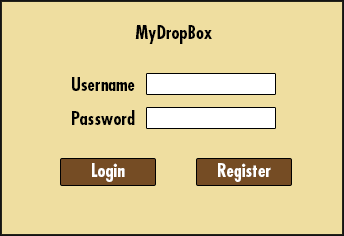
\includegraphics[width=250pt]{screen.png}}}
		\vspace{1em}
	\end{figure}


	The application will be designed in \textit{C++}. The user interaction of the application will be supported by \textit{Qt}. Network communication will happen over \textit{Sockets}. Both client and server applications will be Desktop applications, with proper interface wherever necessary.

	\section{Features}
		\subsection{Sharing}
			Each user will have a designated a username and password along with some amount of space upon registration. This can be used to login to the application and connect with the server. The files will be uploaded via the Desktop application to the server by the user.\\

			The uploaded file(s) may be shared with other MyDropBox users with proper access permissions like Read and Write. Upload and Download will happen over TCP sockets. Sharing information is saved both on server and local system in a separate Hidden Folder (similar to Git).

		\subsection{Synchronization}
			The contents of the server shall be synced with Desktop application both at Re-Login and File Upload/Download. The contents shall be saved locally as well. The sync will happen on the basis of Last Updated Timestamps of Files shared by a single user. Files updated / uploaded after the time of last sync will be updated. The timestamps will be accessed by C++ \textit{stat} command.

		\subsection{File Hashing}
			Every file will be MD5-hashed at the upload. If a file with the same MD5 hash exists on the server, it need not be uploaded again. All the files on the server shall be saved at a single location with an index table (stored in a separate file) to associate each file to a user. The hash shall be calculated using \textit{OpenSSL Digest Functions}.

		\subsection{File History}
			The user(s) shall have the option of updating the files whenever needed. All the revisions can be accessed and downloaded via the client application. The information about the revision history will be saved in the same hidden folder containing the sharing information, on the local machine.\\
			
			The revisions will work similar to the Git update system i.e. when a file is updated, just the updates and the update positions are stored along with base file. The difference will be analysed using the \textit{google-diff-match-patch} library.

		\subsection{SSL Encryption}
			The data would flow over secure SSL connections. The certificate(s) for connection would be generated using OpenSSH with a 2048 bit Key. This would help prevent the Man-in-the-middle attacks on MyDropBox.

		\subsection{Local Persistent Storage}
			The files shared on MyDropBox will be synced locally to a folder on user's machine (from where the user logins to the application), similar to \textbf{Google Drive} and \textbf{OneDrive}. Whenever the user re-logins on the machine and/or updates a file in his space, the contents of the local folder are re-synced with the server. This allows saving the bandwidth as well as better efficiency in terms of file sharing.

	\endgroup

\end{document}